\documentclass{beamer}

\usepackage{subcaption}
\usepackage{tikz}
\usepackage{multicol}
\usetikzlibrary{calc}
\usetikzlibrary{decorations.pathreplacing}

\usepackage[backend=biber, backref=true, firstinits=true, url=true, isbn=true]{biblatex}
\addbibresource{present.bib}

\usetheme{Singapore}
\usefonttheme[onlymath]{serif}
\setbeamertemplate{navigation symbols}{}
\date{}

\renewcommand{\ss}{\scriptscriptstyle}

\title{Polynomial Chaos}
\author{Alex Carney \\ C1338020}

\begin{document}

\begin{frame}
    \titlepage
    \begin{figure}
        \centering
        
\includegraphics[width=0.25\linewidth]{img/universitylogo-eps-converted-to.pdf}
    \end{figure}
\end{frame}

\section{Introduction}

\begin{frame}
    \frametitle{Introduction}

    \pause
    \begin{itemize}
        \item $u_t - \Delta u = 0$
        \pause
        \item $u_{tt} - c^2\Delta u = 0$
        \pause
        \item $-\Delta u = f$
    \end{itemize}
\end{frame}

\section{Deterministic Case}
\begin{frame}
    \begin{itemize}
        \item For $x \in [0,1]$ $$-au''(x) + bu'(x) + cu(x) = f(x)$$
        \item $u(0) = u(1) = 0$
    \end{itemize}
\end{frame}

\begin{frame}
    \begin{align*}
        a\int_0^1u'(x)v'(x)\, dx + b\int_0^1&u'(x)v(x)\, dx + c\int_0^1cu(x)v(x)\, dx \\
                                            &= \int_0^1f(x)v(x)\, dx
    \end{align*}

    $u(x)$ is a solution if the above holds $\forall v \in H_0^1([0,1])$
\end{frame}

\begin{frame}

    \begin{figure}
        \centering
        \begin{tikzpicture}[scale=4.0]
            \draw (-1, 0) -- (1, 0);
            \draw (-1, 0.02) -- (-1, -0.02);
            \draw (1, 0.02) -- (1, -0.02);

            \node (0) at (-1, 0.1) {$0$};
            \node (1) at (1, 0.1) {$1$};

        \end{tikzpicture}
    \end{figure}
\end{frame}

\begin{frame}

    \begin{figure}
        \centering
        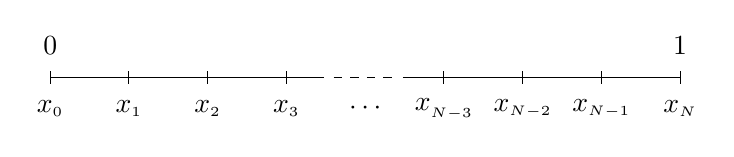
\begin{tikzpicture}[scale=4]
            % Draw the 0-1 interval
            \draw (-1,0) -- (-0.13, 0);
            \draw[dashed] (-0.1, 0) -- (0.1, 0);
            \draw (0.12, 0) -- (1, 0);

            \draw (-1, 0.02) -- (-1, -0.02);
            \node (x0) at (-1, -0.1) {$x_{\ss 0}$};

            \draw (-0.75, 0.02) -- (-0.75, -0.02);
            \node (x1) at (-0.75, -0.1) {$x_{\ss 1}$};

            \draw (-0.5, 0.02) -- (-0.5, -0.02);
            \node (x2) at (-0.5, -0.1) {$x_{\ss 2}$};

            \draw (-0.25, 0.02) -- (-0.25, -0.02);
            \node (x3) at (-0.25, -0.1) {$x_{\ss 3}$};

            \node (d) at (0,-0.1) {$\cdots$};

            \draw (0.25, 0.02) -- (0.25, -0.02);
            \node (xn3) at (0.25, -0.1) {$x^{}_{\ss N-3}$};

            \draw (0.5, 0.02) -- (0.5, -0.02);
            \node (xn2) at (0.5, -0.1) {$x_{\ss N-2}$};

            \draw (0.75, 0.02) -- (0.75, -0.02);
            \node (xn1) at (0.75, -0.1) {$x_{\ss N-1}$};

            \draw (1, 0.02) -- (1, -0.02);
            \node (xN) at (1, -0.1) {$x_{\ss N}$};

            % Draw the 0, 1 labels
            \node () at (-1, 0.1) {0};
            \node () at (1, 0.1) {1};

        \end{tikzpicture}
    \end{figure}
\end{frame}

\begin{frame}

    \begin{figure}
        \centering
        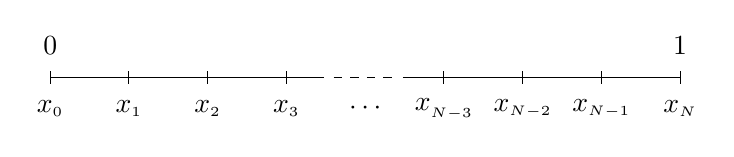
\begin{tikzpicture}[scale=4]
            % Draw the 0-1 interval
            \draw (-1,0) -- (-0.13, 0);
            \draw[dashed] (-0.1, 0) -- (0.1, 0);
            \draw (0.12, 0) -- (1, 0);

            \draw (-1, 0.02) -- (-1, -0.02);
            \node (x0) at (-1, -0.1) {$x_{\ss 0}$};

            \draw (-0.75, 0.02) -- (-0.75, -0.02);
            \node (x1) at (-0.75, -0.1) {$x_{\ss 1}$};

            \draw (-0.5, 0.02) -- (-0.5, -0.02);
            \node (x2) at (-0.5, -0.1) {$x_{\ss 2}$};

            \draw (-0.25, 0.02) -- (-0.25, -0.02);
            \node (x3) at (-0.25, -0.1) {$x_{\ss 3}$};

            \node (d) at (0,-0.1) {$\cdots$};

            \draw (0.25, 0.02) -- (0.25, -0.02);
            \node (xn3) at (0.25, -0.1) {$x^{}_{\ss N-3}$};

            \draw (0.5, 0.02) -- (0.5, -0.02);
            \node (xn2) at (0.5, -0.1) {$x_{\ss N-2}$};

            \draw (0.75, 0.02) -- (0.75, -0.02);
            \node (xn1) at (0.75, -0.1) {$x_{\ss N-1}$};

            \draw (1, 0.02) -- (1, -0.02);
            \node (xN) at (1, -0.1) {$x_{\ss N}$};

            % Draw the 0, 1 labels
            \node () at (-1, 0.1) {0};
            \node () at (1, 0.1) {1};

        \end{tikzpicture}
    \end{figure}

    \begin{align*}
        u^h(x) = \sum_{j=0}^Nu_j\phi_j(x) &&
        f(x) \approx \sum_{j=0}^Nf_j\phi_j(x)
    \end{align*}
\end{frame}

\begin{frame}

    \begin{figure}
        \centering
        \begin{tikzpicture}[scale=4]
            % Draw the 0-1 interval
            \draw (-1,0) -- (-0.13, 0);
            \draw[dashed] (-0.1, 0) -- (0.1, 0);
            \draw (0.12, 0) -- (1, 0);

            \draw (-1, 0.02) -- (-1, -0.02);
            \node (x0) at (-1, -0.1) {$x_{\ss 0}$};

            \draw (-0.75, 0.02) -- (-0.75, -0.02);
            \node (x1) at (-0.75, -0.1) {$x_{\ss 1}$};

            \draw (-0.5, 0.02) -- (-0.5, -0.02);
            \node (x2) at (-0.5, -0.1) {$x_{\ss 2}$};

            \draw (-0.25, 0.02) -- (-0.25, -0.02);
            \node (x3) at (-0.25, -0.1) {$x_{\ss 3}$};

            \node (d) at (0,-0.1) {$\cdots$};

            \draw (0.25, 0.02) -- (0.25, -0.02);
            \node (xn3) at (0.25, -0.1) {$x^{}_{\ss N-3}$};

            \draw (0.5, 0.02) -- (0.5, -0.02);
            \node (xn2) at (0.5, -0.1) {$x_{\ss N-2}$};

            \draw (0.75, 0.02) -- (0.75, -0.02);
            \node (xn1) at (0.75, -0.1) {$x_{\ss N-1}$};

            \draw (1, 0.02) -- (1, -0.02);
            \node (xN) at (1, -0.1) {$x_{\ss N}$};

            % Draw the 0, 1 labels
            \node () at (-1, 0.1) {0};
            \node () at (1, 0.1) {1};

            \node () at (-0.75, 0.55) {$\color{red}\phi_1(x)$};

            \draw[red] (-1, 0) -- (-0.75, 0.5) -- (-0.5, 0);

        \end{tikzpicture}
    \end{figure}

    \begin{align*}
        u^h(x) = \sum_{j=0}^Nu_j\phi_j(x) &&
        f(x) \approx \sum_{j=0}^Nf_j\phi_j(x)
    \end{align*}
\end{frame}

\begin{frame}
    \[
        A\mathbf{u} = M\mathbf{f}
    \]
    \begin{itemize}
        \item $A_{i,j} = a\int\phi_i'\phi_j'\ dx + b\int\phi_i\phi_j'\ dx
                    + c\int\phi_i\phi_j\ dx$
        \item $M_{i,j} = \int\phi_i\phi_j\, dx$
    \end{itemize}
\end{frame}

\begin{frame}
    \begin{figure}
    \centering
    \begin{subfigure}[b]{0.45\textwidth}
        \centering
        \resizebox{\linewidth}{!}{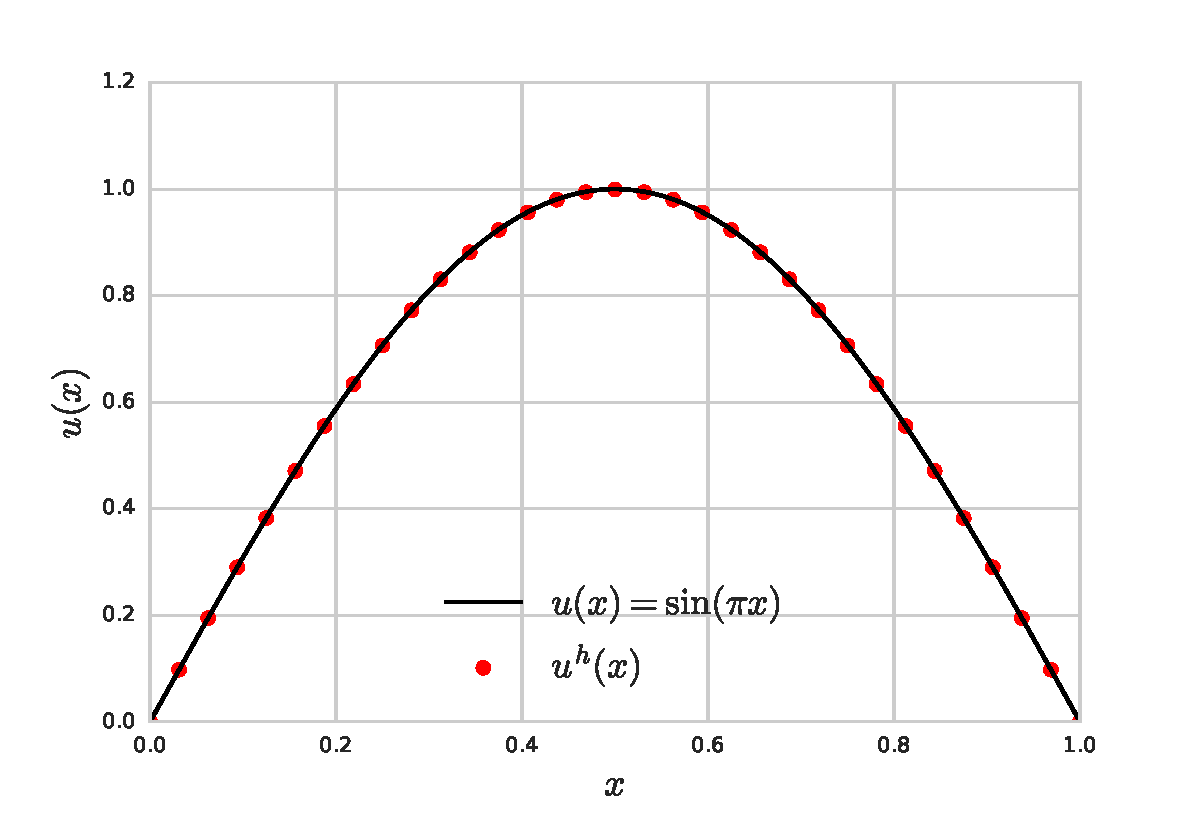
\includegraphics{img/oned-deterministic-plot.pdf}}
    \end{subfigure}
    \begin{subfigure}[b]{0.45\textwidth}
        \centering
        \resizebox{\linewidth}{!}{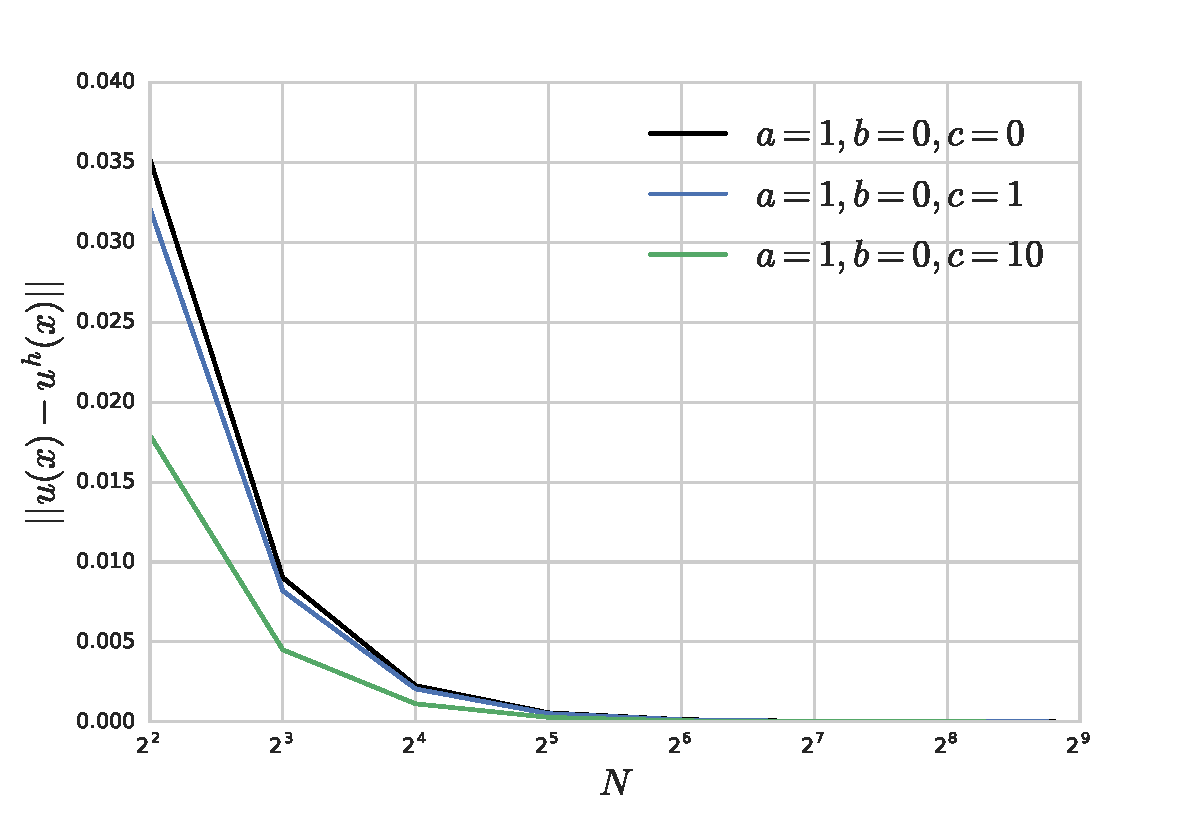
\includegraphics{img/one-d-deterministic-error.pdf}}
    \end{subfigure}
    \end{figure}

    \begin{itemize}
        \item $a = 1, b = 0, c = 0$ and $f(x) = \pi^2\sin{(\pi x)}$
        \item $a = 1, b = 0, c = 1$ and $f(x) = \pi^2\sin{(\pi x)} + \sin{(\pi x)}$
        \item $a = 1, b = 2, c= 0$ and $f(x) = \pi^2\sin{(\pi x)} + 2\pi\cos{(\pi x)}$
    \end{itemize}
\end{frame}

\section{Stochastic Case}
\begin{frame}
    \begin{itemize}
        \item For $x \in [-1,1]$ and $\omega \in \Omega$
            $$-\frac{d}{dx}\left[a(x;\omega)\frac{d}{dx}u(x;\omega)\right] = f(x)$$
        \item $u(-1;\omega) = u(1;\omega) = 0$
    \end{itemize}

    \pause

    \begin{itemize}
        \item ``Modelling uncertainty in steady state diffusion problems via
                generalised polynomial chaos'' - D.Xiu and G.E. Karniadakis
    \end{itemize}

\end{frame}

\begin{frame}
    \begin{align*}
        \int_\Omega\int_{-1}^1a(x;\omega)\frac{d}{dx}&u(x;\omega)\frac{d}{dx}w(x;\omega)\
        dx\ d\Omega \\ &= \int_\Omega\int_{-1}^1f(x)w(x;\omega)\ dx\ d\Omega
    \end{align*}

    $u(x)$ is a solution if the above holds $\forall v \in H_0^1([-1,1])\times
    L^2(\Omega)$
\end{frame}

\begin{frame}
    \[
        X(\mathbf{x};\omega) = \bar{X}(\mathbf{x})
         + \sum_{n=0}^\infty\sqrt{\lambda_n}\beta_n(\mathbf{x})\xi_n(\omega)
    \]
    \pause
    \[
        \int_DC(\mathbf{x}_1, \mathbf{x}_2)\beta(\mathbf{x}_1)\ d\mathbf{x}_1
            = \lambda\beta(\mathbf{x}_2)
    \]
\end{frame}

\begin{frame}
    \[
        a(x;\omega) = 1 + \epsilon\kappa(x;\omega)
    \]
    \pause
    \[
        C(x,y) = \sigma^2\exp\left(-\frac{|x - y|}{k}\right)
    \]
    \pause
    \[
        \sigma^2\int_{-1}^1\exp(-|x - y|)\beta_n(y)\ dy = \lambda_n\beta_n(x)
    \]
\end{frame}

\begin{frame}
    \begin{figure}
        \centering
        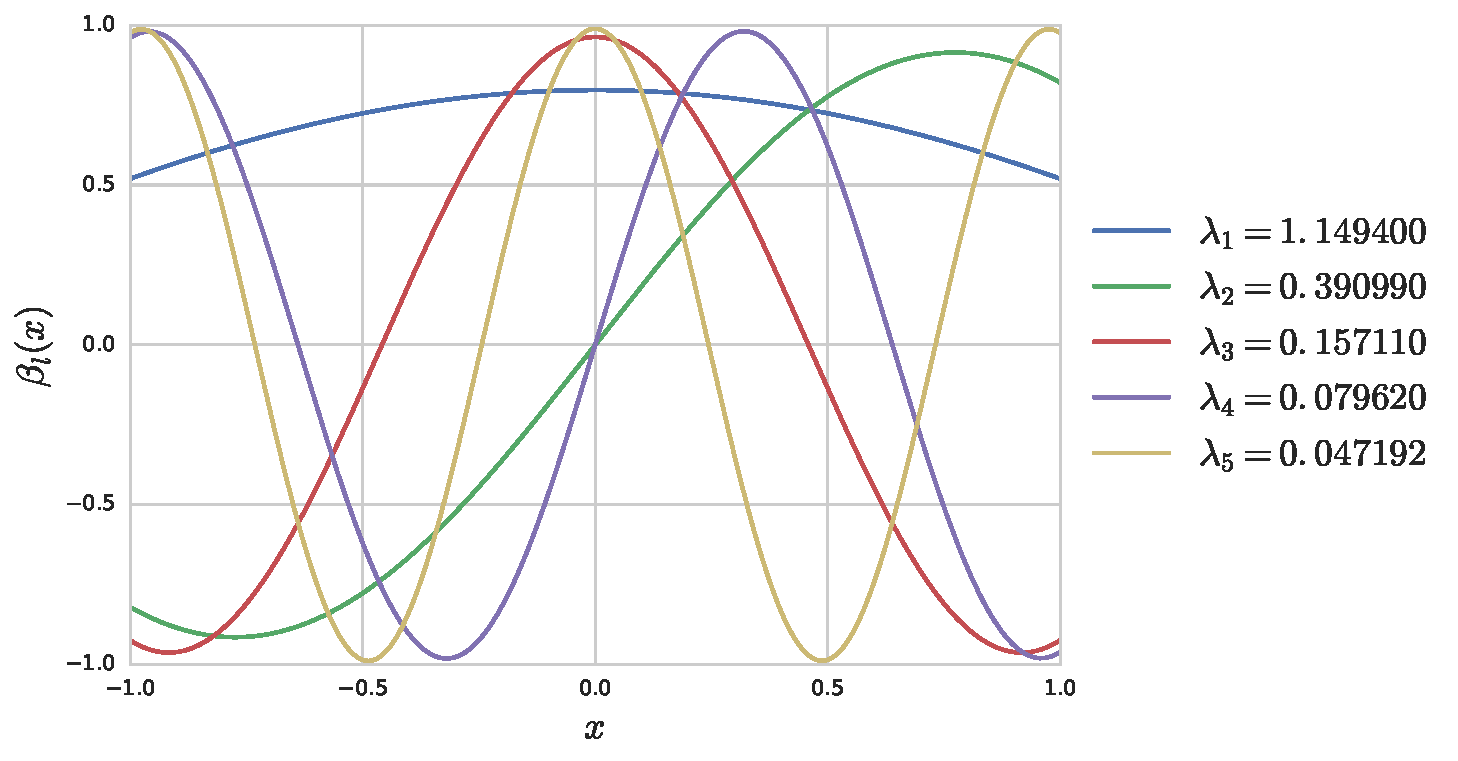
\includegraphics[width=0.75\linewidth]{img/kle-eigenfunctions.pdf}
    \end{figure}
    \pause
    \[
        a(x;\omega) \approx 1 + \epsilon\left(\mu
            + \sigma^2\sum_{l=1}^d\sqrt{\lambda_l}\beta_l(x)\xi_l(\omega)\right)
    \]
\end{frame}

\begin{frame}
    \[
        \begin{array}{c c c}
            \alpha_1 = (0,0) & \alpha_2 = (1,0) & \alpha_3 = (0,1) \\
            \alpha_4 = (2,0) & \alpha_5 = (1,1) & \alpha_6 = (0,2)
        \end{array}
    \]
    \pause
    \[
        \begin{array}{c c c}
            \chi_{\alpha_1} = 1 & \chi_{\alpha_2} = \xi_1 & \chi_{\alpha_3} = \xi_2 \\
            \chi_{\alpha_4} = \frac{1}{2}(3\xi_1^2 - 1) &
            \chi_{\alpha_5} = \xi_1\xi_2 &
            \chi_{\alpha_6} = \frac{1}{2}(3\xi_2^2 - 1)
        \end{array}
    \]
    \pause
    \[
        u^{h,P}(x;\omega) = \sum_{j=0}^N\sum_{s=1}^Pu_{j,s}\chi_s(\xi)\phi_j(x)
    \]
    \[
        P = \frac{(d+p)!}{d!p!}
    \]
\end{frame}

\begin{frame}
    \[
        \begin{array}{l r}
        A = \left[\begin{array}{c c c}
            A_{1,1} & \cdots & A_{1,P} \\
            \vdots & & \vdots \\
            A_{P,1} & \cdots & A_{P,P}
        \end{array}\right]&
        M = \left[\begin{array}{c}
            M_1 \\ \vdots \\ M_P
        \end{array}\right]
    \end{array}
    \]
    \pause
    \[
        (A_{s,s})_{i,j} = (1 + \epsilon\mu)\langle\langle\chi_s^2\rangle\rangle
        \int\phi_j'\phi_i'\ dx
    \]
    \pause
    \[
        (A_{s,t})_{i,j} = \epsilon\sigma^2\sum_{l=1}^d\sqrt{\lambda_l}
            \langle\langle\xi_l\chi_s\chi_t\rangle\rangle
            \int\beta_l\phi_j'\phi_i'\ dx
    \]
    \pause
    \[
        (M_t)_{i,j} = \langle\langle\chi_t\rangle\rangle\int\phi_j\phi_i\ dx
    \]
\end{frame}

\begin{frame}
    \[
        \begin{array}{l r}
        A = \left[\begin{array}{c c c}
            A_{1,1} & \cdots & A_{1,P} \\
            \vdots & & \vdots \\
            A_{P,1} & \cdots & A_{P,P}
        \end{array}\right]&
        M = \left[\begin{array}{c}
                M_1 \\ \mathbf{0} \\ \vdots \\ \mathbf{0}
        \end{array}\right]
    \end{array}
    \]
    \[
        (A_{s,s})_{i,j} = (1 + \epsilon\mu)\langle\langle\chi_s^2\rangle\rangle
        \int\phi_j'\phi_i'\ dx
    \]
    \[
        (A_{s,t})_{i,j} = \epsilon\sigma^2\sum_{l=1}^d\sqrt{\lambda_l}
            \langle\langle\xi_l\chi_s\chi_t\rangle\rangle
            \int\beta_l\phi_j'\phi_i'\ dx
    \]
    \[
        (M_t)_{i,j} = \langle\langle\chi_t\rangle\rangle\int\phi_j\phi_i\ dx
    \]
\end{frame}

\begin{frame}
    \begin{figure}
        \centering
        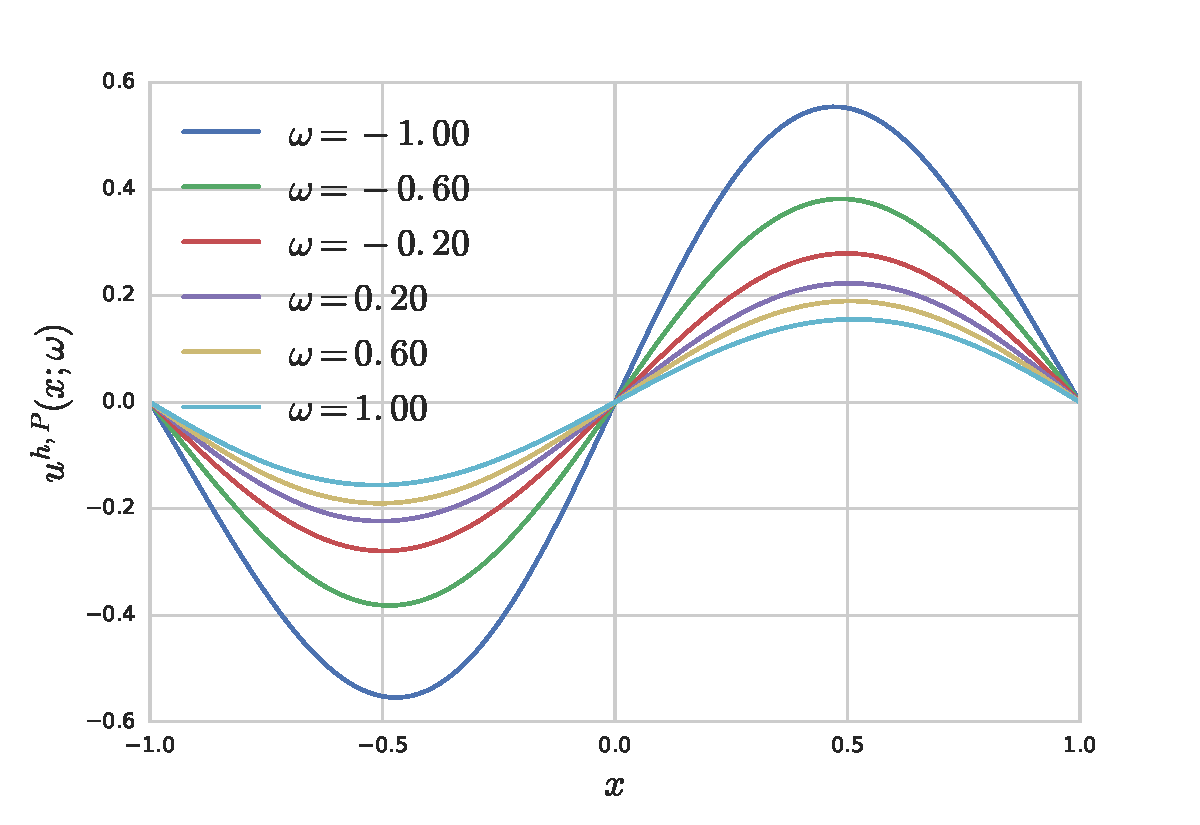
\includegraphics[width=0.75\linewidth]{img/oned-stochastic-realisations-1-3.pdf}
        \caption{$\epsilon = 1$, $d = 1$, $p = 3$}
    \end{figure}
\end{frame}

\begin{frame}
    \[
        u_{j,s} = \left[\begin{array}{c c c}
                        u_{1,1} & \cdots & u_{1,P} \\
                        \vdots & & \vdots \\
                        u_{N,1} & \cdots & u_{N, P}
                     \end{array}\right]
    \]
    \pause
    \begin{align*}
        \mathbb{E}[u^{h,P}] &= \sum_{j=0}^Nu_{j,s}\phi_j(x)\sum_{s=1}^P\int_\Omega\chi_s\ d\Omega \\
                            &= \sum_{j=0}^Nu_{j,1}\phi_j(x)
    \end{align*}
\end{frame}

\begin{frame}
    \begin{figure}
        \centering
        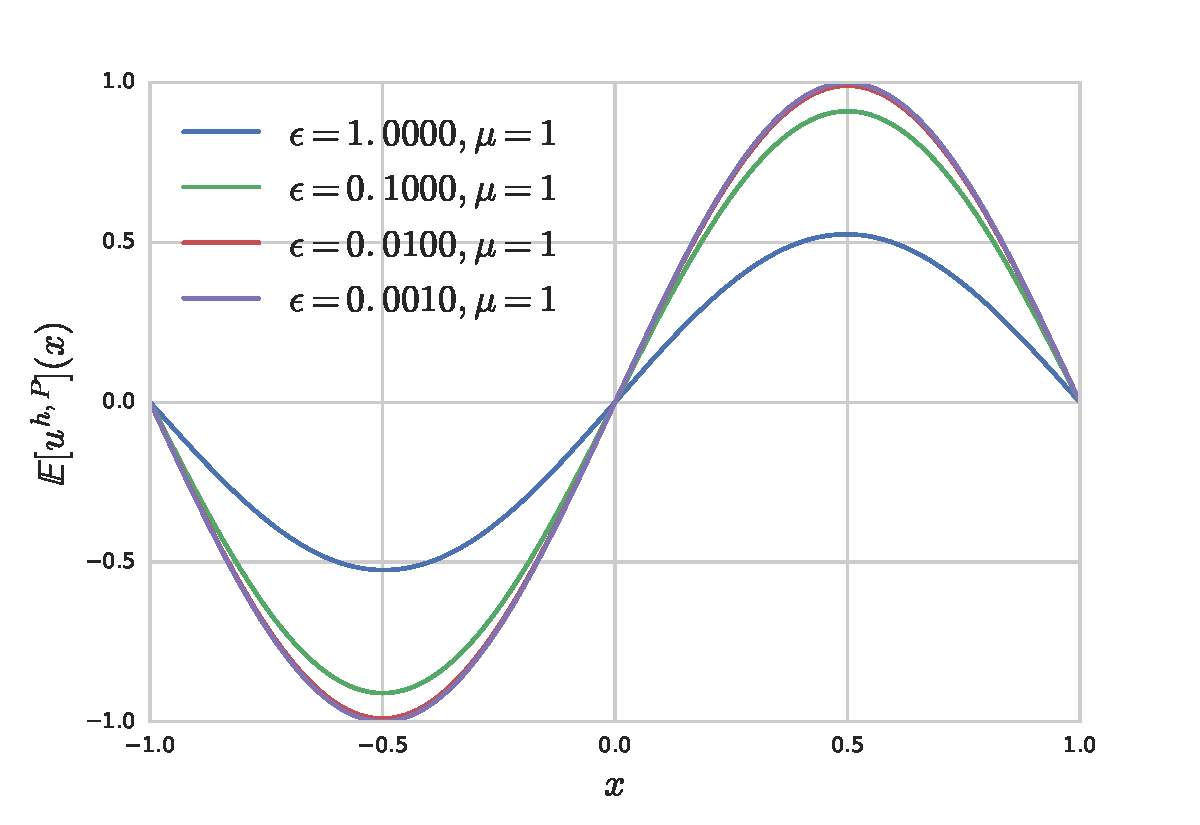
\includegraphics[width=0.75\linewidth]{img/oned-stochastic-mean-soln-process.pdf}
    \end{figure}
\end{frame}

\begin{frame}
    \[
        Var(u^{h,P}) = \mathbb{E}\left[(u^{h,P})^2\right] - (\mathbb{E}[u^{h,P}])^2
    \]
\end{frame}

\begin{frame}
    \begin{figure}
        \centering
        \begin{subfigure}[b]{0.45\linewidth}
            \centering
            \resizebox{\linewidth}{!}{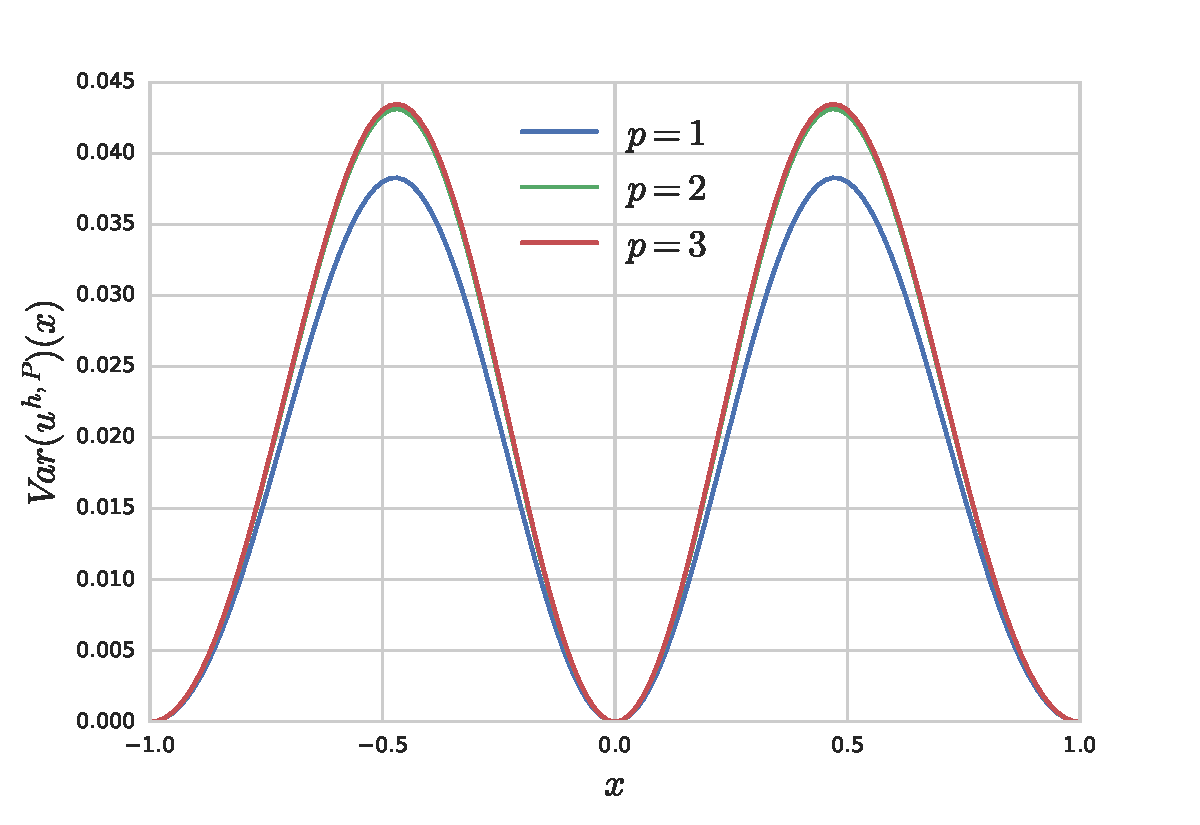
\includegraphics{img/oned-stochastic-variance-plots.pdf}}
        \end{subfigure}
        \begin{subfigure}[b]{0.45\linewidth}
            \centering
            \resizebox{\linewidth}{!}{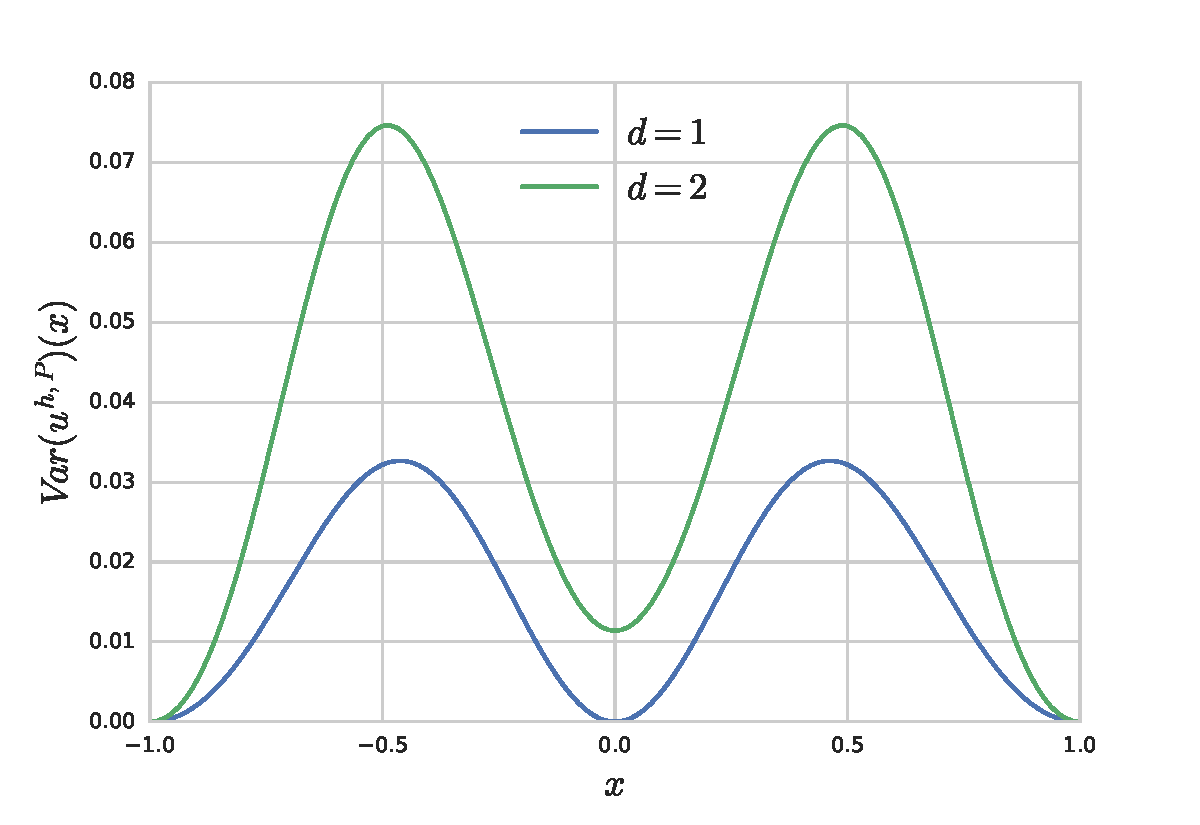
\includegraphics{img/oned-stochastic-variance-plots-d.pdf}}
        \end{subfigure}
    \end{figure}
\end{frame}

\begin{frame}
    \begin{figure}
        \centering
        \begin{subfigure}[b]{0.45\linewidth}
            \centering
            \resizebox{\linewidth}{!}{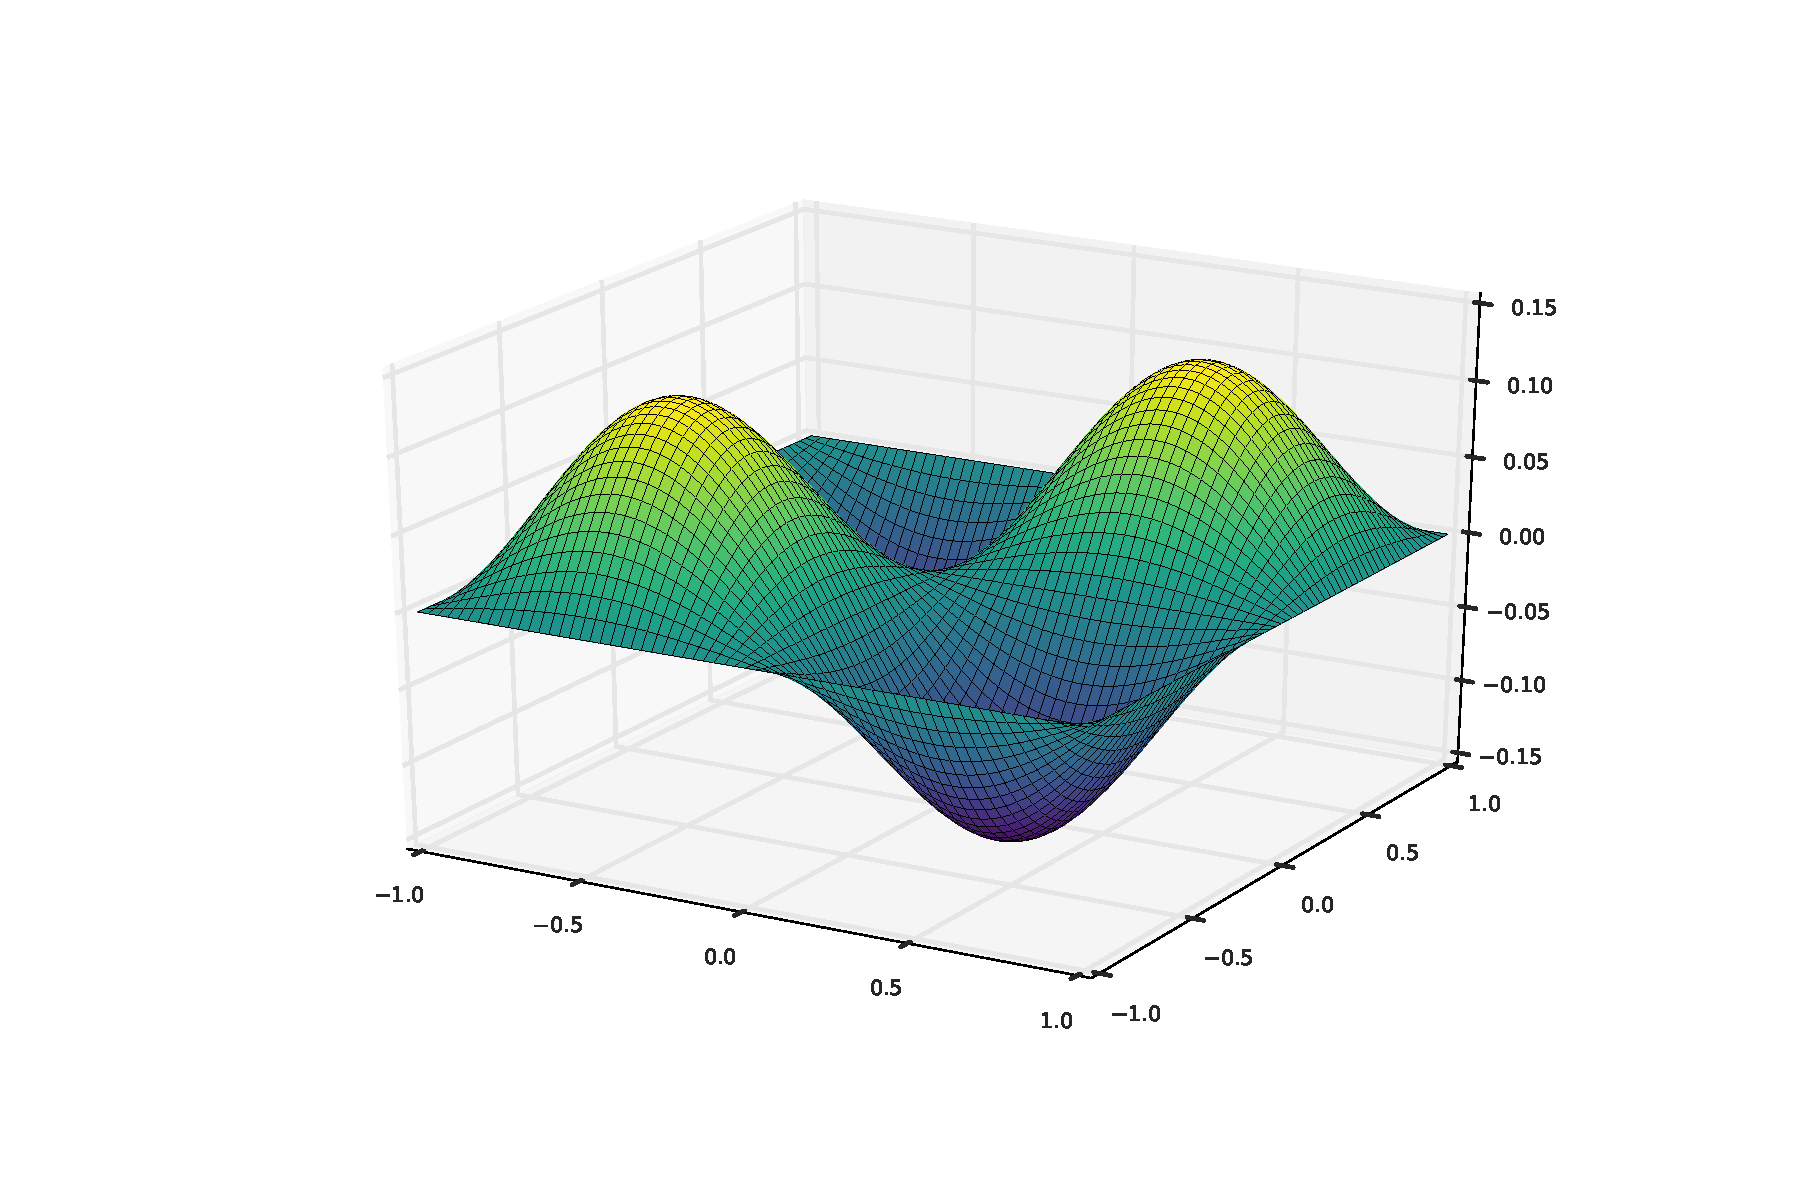
\includegraphics{img/twod-stochastic-mean-surface.pdf}}
        \end{subfigure}
        \begin{subfigure}[b]{0.45\linewidth}
            \centering
            \resizebox{\linewidth}{!}{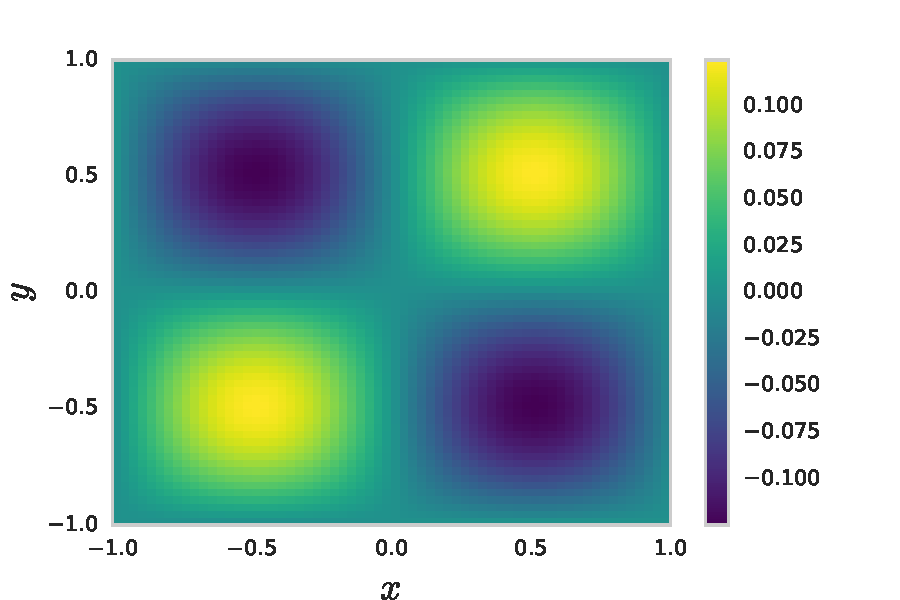
\includegraphics{img/twod-stochastic-mean-heat.pdf}}
        \end{subfigure}
    \end{figure}
    \begin{figure}
        \centering
        \begin{subfigure}[b]{0.45\linewidth}
            \centering
            \resizebox{\linewidth}{!}{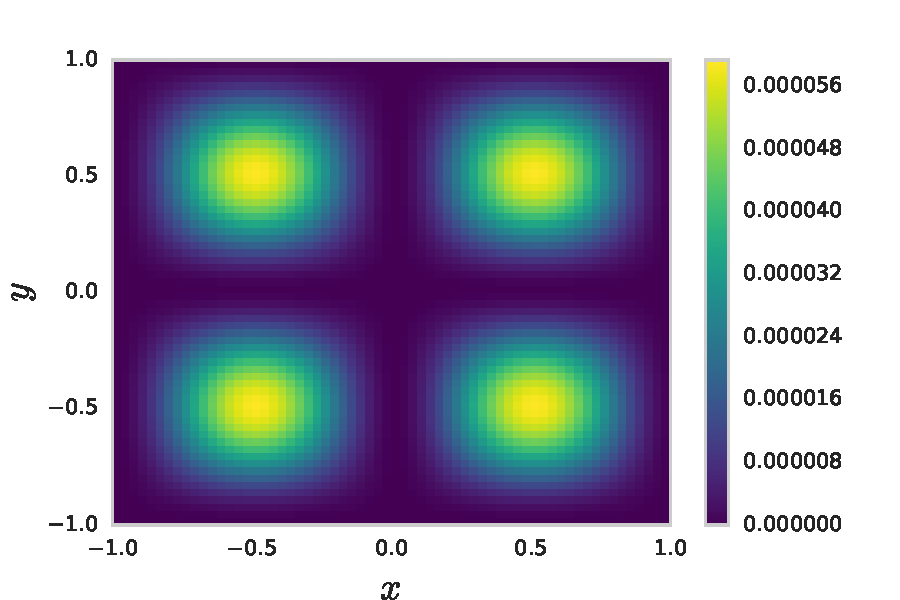
\includegraphics{img/twod-stochastic-variance-heat.pdf}}
        \end{subfigure}
        \begin{subfigure}[b]{0.45\linewidth}
            \centering
            \resizebox{\linewidth}{!}{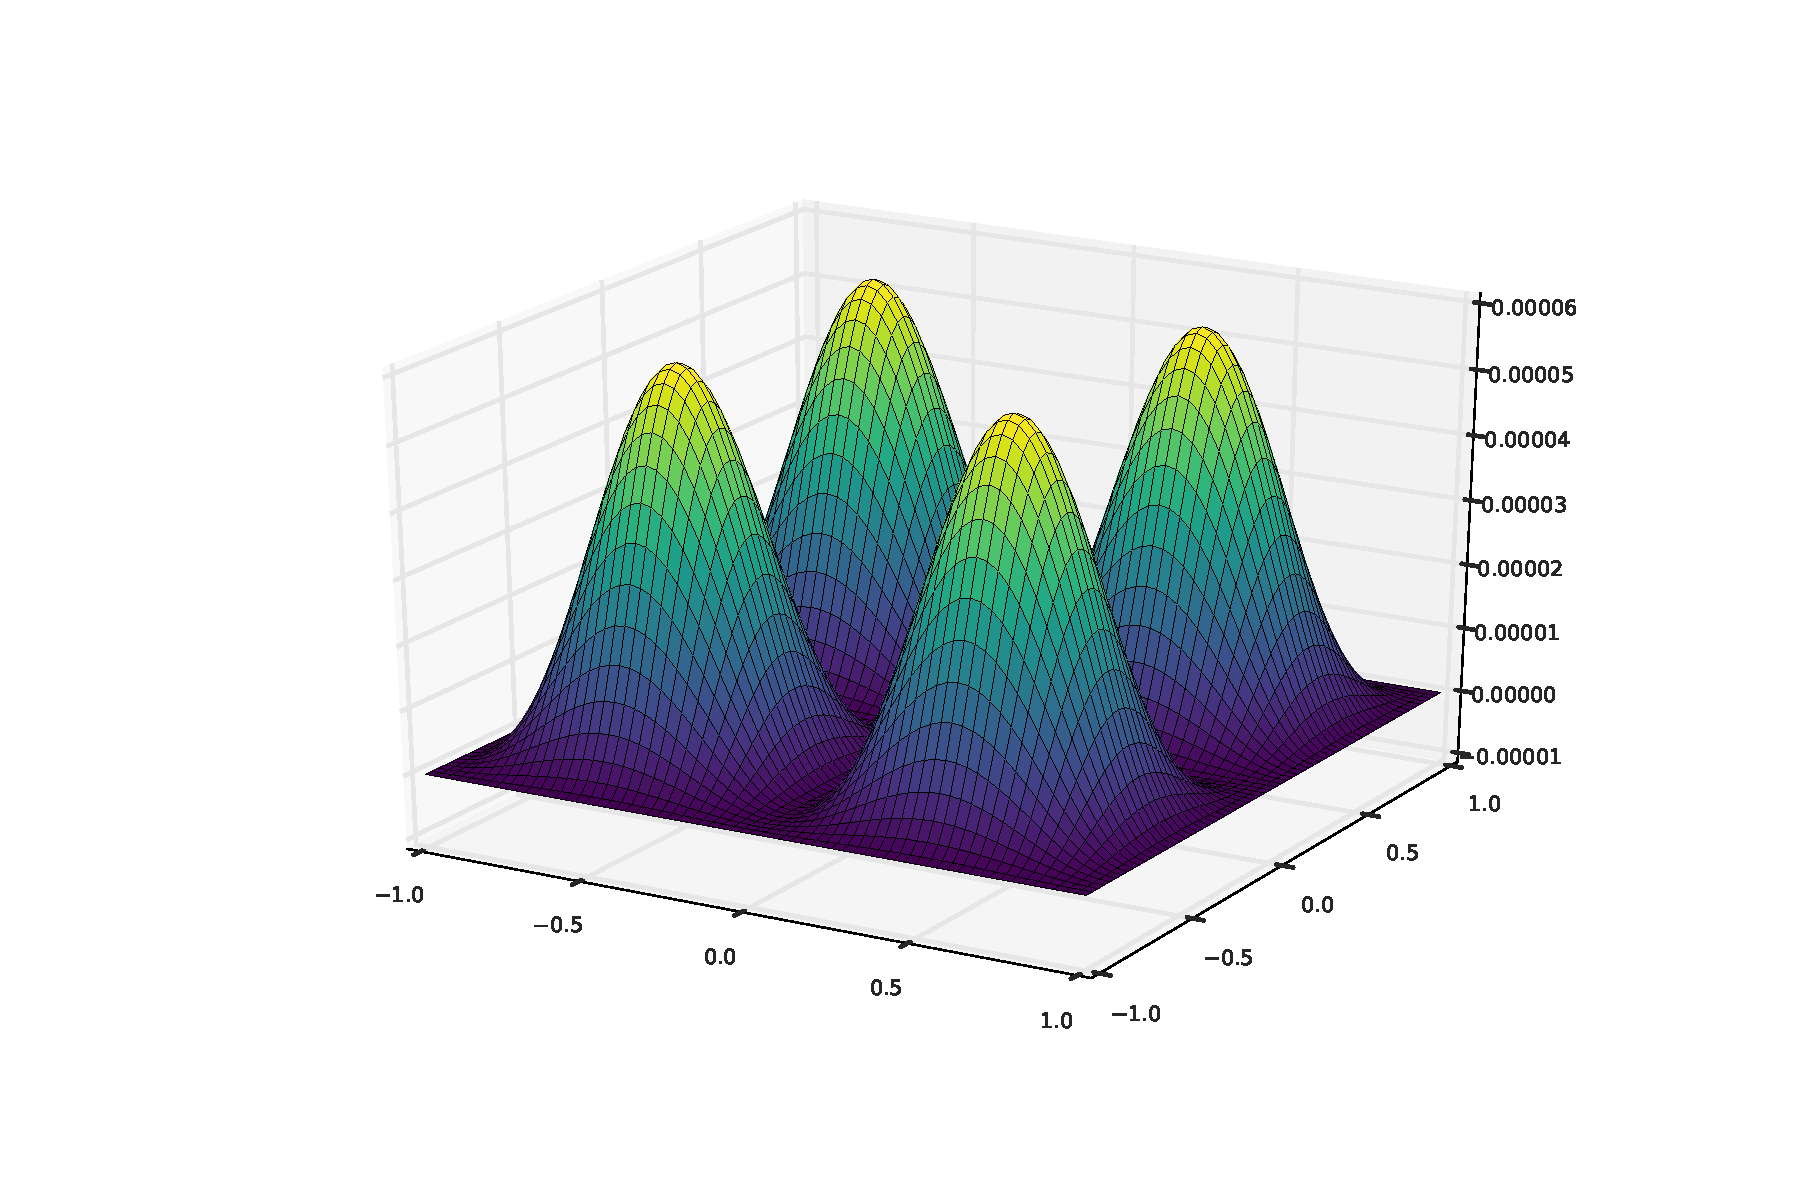
\includegraphics{img/twod-stochastic-variance-surface.pdf}}
        \end{subfigure}
    \end{figure}
\end{frame}

\end{document}
